\documentclass[working, oneside]{inputs/tuftebook}
\usepackage[utf8]{inputenc}
\usepackage[T1]{fontenc}
\usepackage{textcomp}

\usepackage{url}

\usepackage[
    sorting=nyt,
    style=alphabetic
]{biblatex}
\addbibresource{bibliography.bib}

\usepackage{hyperref}
\hypersetup{
    colorlinks,
    linkcolor={black},
    citecolor={black},
    urlcolor={blue!80!black}
}
\usepackage[noabbrev]{cleveref}

% Adds Bibliography, ... to Table of Contents
\usepackage[nottoc]{tocbibind}

\usepackage{graphicx}
\usepackage{float}
\usepackage[usenames,dvipsnames,svgnames]{xcolor}

% \usepackage{cmbright}

\usepackage{amsmath, amsfonts, mathtools, amsthm, amssymb}
\usepackage{mathrsfs}
\usepackage{cancel}

\newcommand\N{\ensuremath{\mathbb{N}}}
\newcommand\R{\ensuremath{\mathbb{R}}}
\newcommand\Z{\ensuremath{\mathbb{Z}}}
\renewcommand\O{\ensuremath{\emptyset}}
\newcommand\Q{\ensuremath{\mathbb{Q}}}
\newcommand\C{\ensuremath{\mathbb{C}}}
\let\implies\Rightarrow
\let\impliedby\Leftarrow
\let\iff\Leftrightarrow
\let\epsilon\varepsilon

\usepackage{tikz}
\usepackage{tikz-cd}

% theorems
\usepackage{thmtools}
\usepackage{thm-restate}
\usepackage[framemethod=TikZ]{mdframed}
\mdfsetup{skipabove=1em,skipbelow=0em, innertopmargin=12pt, innerbottommargin=8pt}

\theoremstyle{definition}

\makeatletter

\declaretheoremstyle[headfont=\bfseries\sffamily, bodyfont=\normalfont, mdframed={ nobreak } ]{thmgreenbox}
\declaretheoremstyle[headfont=\bfseries\sffamily, bodyfont=\normalfont, mdframed={ nobreak } ]{thmredbox}
\declaretheoremstyle[headfont=\bfseries\sffamily, bodyfont=\normalfont]{thmbluebox}
\declaretheoremstyle[headfont=\bfseries\sffamily, bodyfont=\normalfont]{thmblueline}
\declaretheoremstyle[headfont=\bfseries\sffamily, bodyfont=\normalfont, numbered=no, mdframed={ rightline=false, topline=false, bottomline=false, }, qed=\qedsymbol ]{thmproofbox}
\declaretheoremstyle[headfont=\bfseries\sffamily, bodyfont=\normalfont, numbered=no, mdframed={ nobreak, rightline=false, topline=false, bottomline=false } ]{thmexplanationbox}

\declaretheoremstyle[headfont=\bfseries\sffamily, bodyfont=\normalfont, numbered=no, mdframed={ nobreak, rightline=false, topline=false, bottomline=false } ]{thmexplanationbox}


\declaretheorem[numberwithin=chapter, style=thmgreenbox, name=Definition]{definition}
\declaretheorem[sibling=definition, style=thmredbox, name=Corollary]{corollary}
\declaretheorem[sibling=definition, style=thmredbox, name=Proposition]{prop}
\declaretheorem[sibling=definition, style=thmredbox, name=Theorem]{theorem}
\declaretheorem[sibling=definition, style=thmredbox, name=Lemma]{lemma}
\declaretheorem[sibling=definition, style=thmbluebox,  name=Example]{eg}
\declaretheorem[sibling=definition, style=thmbluebox,  name=Nonexample]{noneg}
\declaretheorem[sibling=definition, style=thmblueline, name=Remark]{remark}




\declaretheorem[numbered=no, style=thmexplanationbox, name=Proof]{explanation}
\declaretheorem[numbered=no, style=thmproofbox, name=Proof]{replacementproof}
\declaretheorem[style=thmbluebox,  numbered=no, name=Exercise]{ex}
\declaretheorem[style=thmblueline, numbered=no, name=Note]{note}

% \renewenvironment{proof}[1][\proofname]{\begin{replacementproof}}{\end{replacementproof}}

% \AtEndEnvironment{eg}{\null\hfill$\diamond$}%

\newtheorem*{uovt}{UOVT}
\newtheorem*{notation}{Notation}
\newtheorem*{previouslyseen}{As previously seen}
\newtheorem*{problem}{Problem}
\newtheorem*{observe}{Observe}
\newtheorem*{property}{Property}
\newtheorem*{intuition}{Intuition}


\declaretheoremstyle[
    headfont=\bfseries\sffamily\color{RawSienna!70!black}, bodyfont=\normalfont,
    mdframed={
        linewidth=2pt,
        rightline=false, topline=false, bottomline=false,
        linecolor=RawSienna, backgroundcolor=RawSienna!5,
    }
]{todo}
\declaretheorem[numbered=no, style=todo, name=TODO]{TODO}


\usepackage{etoolbox}
\AtEndEnvironment{vb}{\null\hfill$\diamond$}%
\AtEndEnvironment{intermezzo}{\null\hfill$\diamond$}%

% http://tex.stackexchange.com/questions/22119/how-can-i-change-the-spacing-before-theorems-with-amsthm
% \def\thm@space@setup{%
%   \thm@preskip=\parskip \thm@postskip=0pt
% }

\usepackage{xifthen}

\makeatother

% figure support (https://castel.dev/post/lecture-notes-2)
\usepackage{import}
\usepackage{xifthen}
\pdfminorversion=7
\usepackage{pdfpages}
\usepackage{transparent}


\makeatletter
\newif\ifworking
\@ifclasswith{tuftebook}{working}{\workingtrue}{\workingfalse}
\makeatother

\newcommand{\incfig}[2][1]{%
    % \ifworking{\makebox[0pt][c]{\color{gray}{\scriptsize\textsf{#2}}}}\fi%
    \def\svgwidth{#1\textwidth}
    \import{./figures/}{#2.pdf_tex}
}

\newcommand{\fullwidthincfig}[2][0.90]{%
    % \ifworking{\makebox[0pt][l]{\color{gray}{\scriptsize\textsf{#2}}}}\fi%
    \def\svgwidth{#1\paperwidth}
    \import{./figures/}{#2.pdf_tex}
}



\newcommand{\minifig}[2]{%
    \def\svgwidth{#1}%
    \begingroup%
    \setbox0=\hbox{\import{./figures/}{#2.pdf_tex}}%
    \parbox{\wd0}{\box0}\endgroup%
    \hspace*{0.2cm}
}

% %http://tex.stackexchange.com/questions/76273/multiple-pdfs-with-page-group-included-in-a-single-page-warning
\pdfsuppresswarningpagegroup=1

\newcommand\todo[1]{\ifworking {{\color{red}{#1}}} \else {}\fi}
\newcommand\charlotte[1]{\ifworking {{\color{blue}{#1}}} \else {}\fi}

\author{Gilles Castel}



\usepackage{multirow}
\def\block(#1,#2)#3{\multicolumn{#2}{c}{\multirow{#1}{*}{$ #3 $}}}

% \overfullrule=1mm

\newenvironment{myproof}[1][\proofname]{%
  \proof[\rm \bf #1]%
}{\endproof}

\usepackage{pdfpages}

\usepackage{lipsum}
\usepackage{parskip}
\usepackage{titletoc}

\usepackage{cmbright}
\usepackage{bm}

\begin{document}
\let\cleardoublepage\clearpage
\section*{Introduction}
In this experiment, we construct a Michelson-Morley interferometer. Our construction a piezoelectric element, which allows for some novel analysis of the setup. We use the setup to test whether a wave-description of light is accurate. 
\section*{Theory}
In this section we will examine the necessary concepts in understanding the michelson-morley interferometer. At its most basic level, we are interested in understanding what happens when light waves collide. In this experiment we will be assuming that the colliding are identical in all aspects expect phase. Their wavelengths and frequencies are identical. Let us assume that our light wave moves along the optical axis, it may then described as,
\[
	\bm{E_i} = E_0 \cos\left( \omega t - kx \right) 
.\] 
\begin{marginfigure}:q
    \centering
    \incfig{fig1}
    \caption{When the light is the incident light hits the beamsplitter, part of it is reflected and the remainder transmitted. Each lightbeam then travels a distance before hitting a mirror. The difference between these distances affects their relative phasedifference. We call it $\Delta s$.}
    \label{fig:fig1}
\end{marginfigure}
Where $\omega$ is the frequency, $k$ the wave number and $E_0$ the amplitude of the wave.When the wave is measured, it has been transmitted and reflected once. We therefore multply the wave amplitude by the coefficients of transmission and reflection, given by the Fresnel Relations.\cite{grif}
 \[
	 \left|\bm{E_i}\right| = \sqrt{RT} \cdot E_0 \cdot \cos\left( \omega t + \rho _i \right) 
.\] 
Where $\rho_i$ is the phase of our wave, at the point where our detector lies. This phase is clearly related to the path length in the following way,
\[
\rho _i  =  \frac{2\pi}{\lambda} S_i
.\]
For our two waves we obtain,
\begin{align*}
	\left|\bm{E_1}\right| = \sqrt{RT} \cdot E_0 \cdot \cos\left( \omega t + \rho _1 \right) \\
	\left|\bm{E_2}\right| = \sqrt{RT} \cdot E_0 \cdot \cos\left( \omega t + \rho _2 \right) 
\end{align*}
Where we have used the fact that transmission and reflection does not impact the frequency of light
If the optics are aligned correctly, we will the be able to measure the overlapping wave on our detector. This wave is given as the sum of $\bm{E_1}$ and $\bm{E_2}$. It's intensity is,
\[
I = c\epsilon_0 \left| \bm{E_1}+\bm{E_2} \right| ^2 = c\epsilon_0RT \left( \cos\left( \omega t +\rho_1 \right) +\cos\left( \omega t +\rho_2 \right)   \right)^2
.\] 
In practice, we are only able to measure the temporal averaging of this, as the frequency is a small quantity. The average of a periodic function with period $\tau$ is,
\[
\left<f \right> = \frac{1}{\tau} \int_{0}^{\tau}f\left( t \right) dt  
.\]
This gives us,
\begin{align*}
\left<I \right> &=  \frac{1}{2\pi} \int_{0}^{2\pi} \left[ \cos\left( \omega t + \rho_1 \right) + \cos\left( \omega t + rho_2 \right)   \right] ^2 d \left( \omega t \right)  \\
&=  1+ \cos\left( \rho _1 - \rho_2  \right)  
.\end{align*}
Now let $ \Delta \rho = \rho_1 - \rho_2$ and also assume that the coeffections of transmissions and reflection equal $0.5$. We then obtain,
 \[
I = \frac{1}{4}c\epsilon_0 E_0^2 \left( 1 + \cos \Delta \rho  \right) 
.\]
\begin{marginfigure}
	\centering
	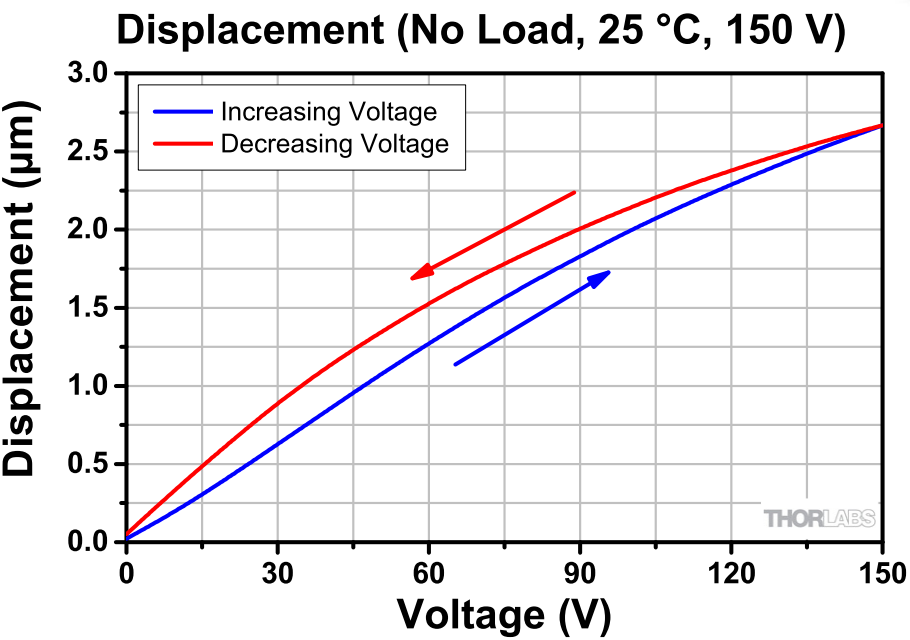
\includegraphics[width=\textwidth]{inputs/piezo}
	\caption{Graph describing til Piezoelement contraction, taken from the Piezo spec-sheet.}
	\label{fig:}
\end{marginfigure}
\section*{Piezoelectric}
We make use of af piezoelectric ring chip, which has the property that it expands when the potential over it increases. This allows us to slightly increase and decrease the path difference the path difference $\Delta s$ in a controlled fashion. The relationship between the potential applied over the piezoelectric and the expansion is nearly linear, as seen in \textbf{fig. 2}. As a result, the path difference should be proportional to the voltage
\[
V \propto \Delta s
\]
\begin{marginfigure}
	\centering
	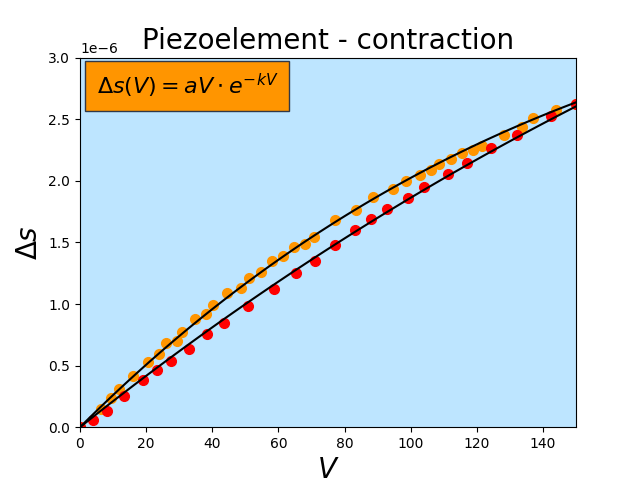
\includegraphics[width=1.1\textwidth]{figures/contraction}
	\caption{Graph of the Piezo-contraction, where $k_C = 2.81\cdot 10^{-3}$,  $a_C = 2.68 \cdot 10^{-8}$. and \\$k_E = 1.40 \cdot 10^{-3}$, $a_E = 2.14 \cdot 10^{-8}$}
	\label{fig:}
\end{marginfigure}
It is particulary smart to change the potential over the piezoelement linearly. By doing this we are able to get displacement from the piezoelement spec-sheet \textbf{fig 2}. The spec-sheet provides a picture of the curve relating potential to displacement. From this picture we were able to extraxt datapoints. The spec-sheet lists the maximum displacement as $2.6 \mu m \pm 15\%$. We have used this $15\%$ as an estimate for the error in our datapoints. We fit these datapoints to determine functional expressions describing the contraction and expansion, $S_C$ and $S_E$. These functions will give half of the path change, as a function of potential. By extensions the phase change will be,
 \[
\Delta \rho_{E /C} \left( V \right) =  \frac{4\pi}{\lambda}S_{E /C}\left( V \right) 
.\] 
An analysis of the spec-sheets yielded the functions $S_E$ and  $S_C$ depicted in \textbf{fig 3.}. These functions will be used when we fit our data the intereferometer.
\section*{Course of action}
For this experiment, we took great care in setting up the interferometer correctly, as the quality of our data solely on this. The laser initially strikes two mirrors, which are used to direct it and correct it horizontally. It then strikes the beam splitter, which is aligned perpendicularly to the ray. The light is then split in two beams of equal intensity. One is transmitted while the other is reflected. These beams then strike mirrors, which send them back towards the beam splitter, where they are gathered and directed towards a detector. Before striking the detector, they pass through a concave lens. This spreads the light more evenly over the sensors in the detector. On one of the mirrors, is mounted a piezoelectric element. Applying a voltage over this element allows us to vary the path distance as the piezoelectric expands and contracts. 
\section*{Results}
In our experiment we measure the induced voltage in the detector as a function of the changing potential over a piezoelectric element. We are interested in relating this changing voltage to the phase change, and thereby ultimately to the path change. In order to figure out how. As the piezoelectric, behaves differently for increasing and decreasing voltagewe have split our data accordingly. For both datasets, we have fit our data to functions of the form,
\[
	I_{E /C} \left( V \right) = A \cos \left( B + \Delta \rho_{E /C}\left( V \right)  \right) +D
.\] 
Where $A$ represents the amplitude of the measured signal and $B, D$ are constant offsets. We are not interested in examining how the detector converts light intensity to signal. We merely check that a constant $A$ is a good description of the fit. We are instead interested in checking whether the base $\cos\left( \Delta \rho  \right) $ is a good description of the data. 
\end{document}
